\documentclass{jsarticle}
\usepackage{amsthm}
\newtheorem{lem}{補題}
\newtheorem{fom}[lem]{公式}
\usepackage{amsmath,amssymb}
\usepackage[dvipdfmx]{graphicx}

\begin{document}


\title{離散構造(後半)レポート}
\author{16B04852 川原和弥}
\date{}
\maketitle


\begin{enumerate}
\setlength{\itemsep}{0.4cm}

\item
\begin{enumerate}
\renewcommand{\labelenumii}{(\arabic{enumii})}
\item $ F - E + V = 0 - 3 + 3  = 0 $
\item $ F - E + V = 1 - 3 + 3  = 1 $
\item $ F - E + V = 0 - 5 + 4  = -1 $
\item $ F - E + V = 1 - 5 + 4  = 0 $
\item $ F - E + V = 1 - 7 + 5  = -1 $
\end{enumerate}


\item
\begin{proof}

まず次の補題\ref{ringoku}を示す。

\begin{lem}[隣国は5つだけ定理]
\label{ringoku}
\begin{eqnarray} どんな地図にも、5個以下の隣国しか持たない国が少なくとも一つは存在する。 \nonumber \end{eqnarray}
\end{lem}

補題\ref{ringoku}の証明. 背理法により証明する。\\
すなわち、すべての国が6個以上の隣国を持つような地図があるとする。\\
この地図の$(面,辺,頂点)$の数を$(F,E,V)$とおくと、
\begin{eqnarray}
1つの頂点に集まる辺は3本以上 \Rightarrow  E \geq \frac{3}{2} V \\
1つの面の境界になる辺は6本以上 \Rightarrow  E \geq \frac{6}{2} F
\end{eqnarray}
また任意の地図上で次の公式\ref{Euler}が成り立つ。
\begin{fom}[Eulerの多面体公式]
\label{Euler}
\begin{eqnarray} F - E + V = 2 \end{eqnarray}
\end{fom}
式(1),(2)より、
\begin{eqnarray}
F - E + V \leq \frac{2}{6} E - E + \frac{2}{3} E = 0 \nonumber
\end{eqnarray}
しかしこれは式(3)に反する。
これにより、すべての国が6個以上の隣国を持つ地図が存在しないことが示された。
\qed \\

以上の補題\ref{ringoku}を踏まえ、問題である$5$色定理を示す。

地図上の国の数$N$に関する帰納法により証明する。
\begin{enumerate}
\item $ N = 1 $のとき\\
任意の色で塗ればよく、自明である。
\item $ N = k $で5色定理が成り立つとする。\\
$ N(M) = k + 1 $である地図$M$を$5$色で塗ることを考える。
補題\ref{ringoku}により$M$には隣国が$5$個以下の国が存在するから、その国を$C(\in M)$とする。
$M$から$C$を除いた地図を$M'(\subsetneq M)$とすると、$ N(M') = k $だから、帰納法の仮定により$M'$は$5$色で塗り分けられる。
\begin{enumerate}
\item $C$が5個の隣国を持ち、全て異なる色で塗られているとき\\
$C$の隣国を時計回りに$C_1,\cdots,C_5$として、それぞれの色を$c_1,\cdots,c_5$とする。
$C_2$から$c_2$と$c_5$のみをたどって到達可能な国の集合を$S(\subsetneq M')$とし、
$C_1$から$c_1$と$c_3$のみをたどって到達可能な国の集合を$S'(\subsetneq M')$とする。
\begin{enumerate}
\item $C_5\notin S$のとき\\
$S$の$c_2$と$c_5$を反転させ、$C$を$c_2$で塗ればよい。
\item $C_5\in S$のとき\\
$S$により$C_1$と$C_3$は分断されているから$C_3\notin S'$である。
したがってA.と同様にして$S'$の$c_1$と$c_3$を反転させ、$C$を$c_1$で塗ればよい。
\end{enumerate}
\item そのほかの場合\\
$C$の隣国に使われていない色で$C$を塗ればよい。\\
\end{enumerate}
\end{enumerate}
(a),(b)より、数学的帰納法から任意の地図上で$5$色定理は肯定される。
\end{proof}

\item
\begin{enumerate}
\renewcommand{\labelenumii}{(\arabic{enumii})}
\item $ w(L_1) = 3 $、$ \langle L_1 \rangle = -A^5 - A^{-3} + A^{-7} $より$ V(L_1) = (-A^3)^{-3}(-A^5 - A^{-3} + A^{-7}) $
\item
ジョーンズ多項式は不変量であり、図形のイソトピーとライマイスター移動に関して不変である。
$L_1$,$L_2$は互いにイソトピックだから
\begin{eqnarray} V(L_2) = V(L_1) = (-A^3)^{-3}(-A^5 - A^{-3} + A^{-7}) \nonumber \end{eqnarray}
\item $ w(L_3) = 0 $、$ \langle L_3 \rangle = A^8 - A^4 + 1 - A^{-4} + A^{-8} $より$ V(L_3) = A^8 - A^4 + 1 - A^{-4} + A^{-8} $
\item
ある結び目$L$とその鏡像$R$のジョーンズ多項式$V(L),V(R)$の関係を考える。\\
まず正交点と負交点が逆転するから\begin{eqnarray} w(R) = - w(L) \end{eqnarray}
そして同様の理由により、カウフマン括弧のルール(K1)の$A$と$A^{-1}$が逆転するから\begin{eqnarray} \langle R \rangle (A) = \langle L \rangle (A^{-1}) \end{eqnarray}
式(4),(5)より
\begin{eqnarray}
V(R)(A) &=& (-A^3)^{-w(R)}\langle R \rangle (A) \nonumber \\
&=& (-(A^{-1})^3)^{-w(L)}\langle L \rangle (A^{-1}) \nonumber \\
&=& V(L)(A^{-1}) \nonumber
\end{eqnarray}
したがって$V(L),V(R)$は$A,A^{-1}$を置き換えた関係にある。\\
$L_4$は$L_3$の鏡像であるから、\begin{eqnarray} V(L_4) = V(L_3)(A^{-1}) = A^8 - A^4 + 1 - A^{-4} + A^{-8} \nonumber \end{eqnarray}
\item
間に交差を挟まないように結び目$L,L'$の和をとる。\\
このとき交点の数はその和となるので、\begin{eqnarray} w(L \times L') = w(L) + w(L') \end{eqnarray}
また$L'$側を固定したまま$L$の方から$\langle L \times L' \rangle$を展開することを考えると、$\langle L \rangle$で最後に残る$\langle \bigcirc \rangle$を$\langle L' \rangle$に置換したものとなるので、
\begin{eqnarray} \langle L \times L' \rangle = \langle L \rangle \langle L' \rangle \end{eqnarray}
式(6),(7)より
\begin{eqnarray}
V(L \times L') &=& (-A^3)^{-w(L \times L')}\langle L \times L' \rangle \nonumber \\
&=& (-A^3)^{-(w(L) + w(L'))}\langle L \rangle \langle L' \rangle \nonumber \\
&=& (-A^3)^{-w(L)}\langle L \rangle (-A^3)^{-w(L')}\langle L' \rangle \nonumber \\
&=& V(L)V(L') \nonumber
\end{eqnarray}
$L_1$の鏡像を$R_1$とすると$L_5 = R_1 \times L_3$であるから、
\begin{eqnarray}
V(L_5) &=& V(R_1 \times L_3) \nonumber \\
&=& V(R_1)V(L_3) \nonumber \\
&=& V(L_1)_{A \to A^{-1}}V(L_3) \nonumber \\
&=& (-A^{-3})^{-3}(-A^{-5} - A^3 + A^7)(A^8 - A^4 + 1 - A^{-4} + A^{-8}) \nonumber \\ \nonumber
\end{eqnarray}
\end{enumerate}

2.\\
\begin{figure}[htbp]
\begin{center}
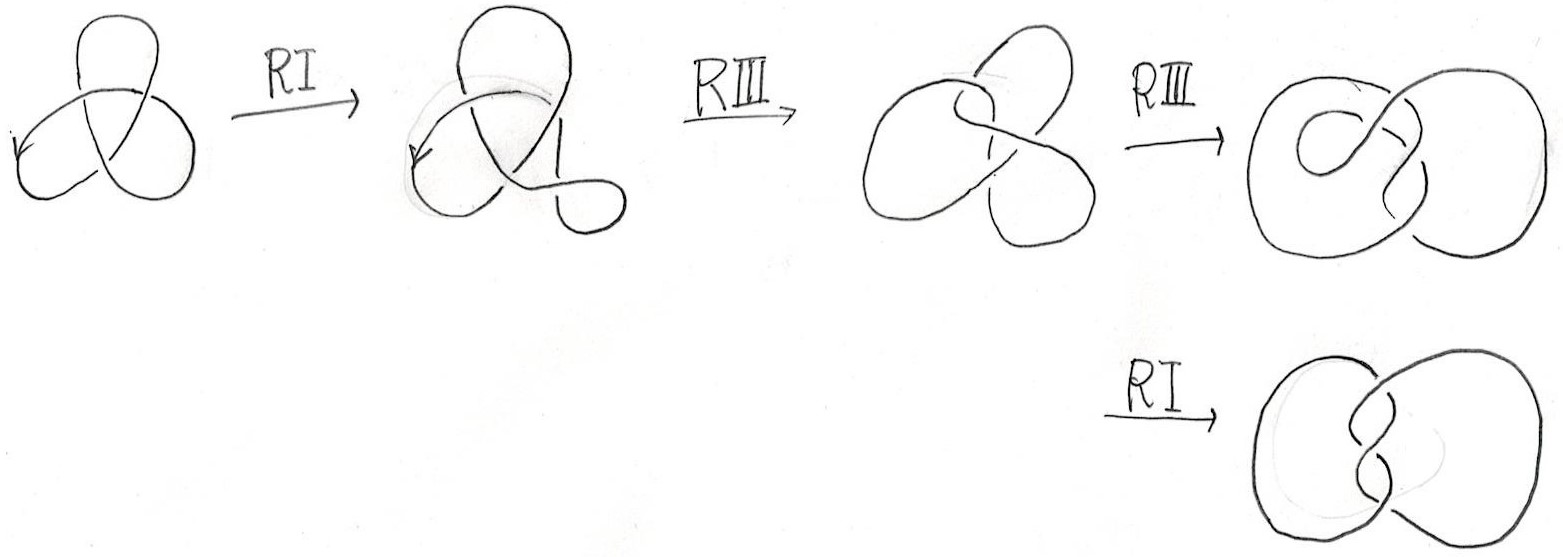
\includegraphics[clip,width=14cm]{2.jpg}
\end{center}
\end{figure}

\end{enumerate}


\end{document}